\chapter{Projektgennemførelse}\label{kapitel_Projektgennemforelse}
I dette afsnit beskrives redskaberne gruppen har anvendt i projektgennemførslen. 

\section{Gruppedannelse}
Gruppen består af Mathias Siig Nørregaard fra IKT, Marie Kirkegaard fra ST og Charlotte Søgaard Kristensen fra ST. 

Gruppensammensætningen er lavet på baggrund af at projektet omhandler både sundhedsfaglige samt tekniske aspekter. I starten var det svært at danne et overblik over den ideelle gruppesammensætning. Det blev valgt at danne gruppen bestående af én IKT-studerende og to ST-studerende: MSN til udvikling af software, samt MK og CSK, til analyser i forhold til det økonomiske perspektiv, konsekvensen af en tilføjelse af ultralyd til screeningsprogrammet, samt en medicinsk godkendelse af Automatisk Ultralydsscanner. 

Gruppen blev ved projektstart enige om at finde en reviewgruppe til feedback af gruppens arbejde. Reviewgruppen består af Jonas Bæch fra ST og Kathrine Duus Kinnerup fra ST med lektor Samuel Alberg Thrysøe som vejleder. Det har fungeret godt at have en reviewgruppe, da reviewgruppen havde forslag til forbedring af bachelorprojektet.  

\section{Samarbejdsaftale}
Ikke alle gruppemedlemmerne kendte hinanden ved projektstart, og det var derfor vigtigt at få lavet en udførlig samarbejdsaftale som dokumentation for gruppens beslutninger og aftaler, samt en rettesnor, hvis der skulle opstå problemer i samarbejdet. 

Det har under projektforløbet ikke været nødvendigt at finde samarbejdsaftalen frem, til konflikthåndtering, da der ingen væsentlige problemer har været med samarbejdet. Samarbejdsaftalen er derfor blevet brugt til forventningsafstemning af projektarbejdet samt til at diskutere forventninger og ønsker til projektarbejdet imellem gruppens medlemmer. 

Samarbejdsaftalen har været et vigtigt redskab for gruppen, da den har været medvirkende til, at problemer i samarbejdet aldrig er opstået. Samarbejdsaftalen er vedlagt i bilag \ref{Samarbejdsaftale} Samarbejdsaftale. 

\section{Arbejdsfordeling}
Arbejdsfordelingen har fungeret godt, og gruppens medlemmer har haft hvert deres ansvarsområde. Arbejdsfordelingen har været opdelt efter kompetencer og interesser hos gruppens medlemmer, samt hvilke fremtidige arbejdsroller gruppens medlemmer kunne se sig selv i.

MSN har primært haft ansvaret for programmeringen af software til Automatisk Ultralydsscanner. MK og CSK har sammen stået for rapportskrivning og brugerundersøgelser, samt risikohåndtering af projektet. MK har haft ansvaret for udarbejdelsen af den medicinske godkendelse, mens CSK har haft ansvaret for den overordnede projektstyring og den økonomiske analyse.

Kravspecifikation, accepttest og design af systemet er diskuteret og udarbejdet i fællesskab, så alle gruppens medlemmer var indforstået med systemets krav og design. Se de udarbejdede bilag i \ref{Kravspecifikation} Kravspecifikation, \ref{Accepttest} Accepttest og \ref{Udviklingsdokument} Dokumentation.

Da bachelorprojektet er et Proof of Concept, har gruppens medlemmer indimellem været udfordret, da mange af opgaverne i projektarbejdet var nyt stof for alle. Her har gruppens medlemmer været gode til at hjælpe og sparre med hinanden, samt til søge hjælp hos vejleder og andre sparringspartnere.  

Nedenstående tabel \ref{ansvarstabel} viser fordelingen af ansvarsområder i gruppen. 

\begin{table}[h]
\centering
\begin{tabular}{|l| p{0.15\textwidth}|}
\hline
\textbf{Ansvarsområde} &  \textbf{Ansvarlig} \\\hline
Kravspecifikation og Accepttest & Fælles \\\hline
Dokumentation & MSN, CSK\\\hline
Brugerundersøgelser & MK, CSK \\\hline
Udvikling af software & MSN\\\hline
Medicinsk godkendelse & MK \\\hline
Overordnet projektstyring & CSK \\\hline
Økonomisk og omkostningseffektiv analyse & CSK \\\hline
\end{tabular}
\caption{Ansvarsområder}
\label{ansvarstabel}
\end{table}

\section{Risikohåndtering af projektarbejdet}
Formålet med risikohåndteringen af projektarbejdet har været at identificere, analysere og evaluere de risici, der kan opstå under arbejdet med bachelorprojektet. Risikohåndteringen er anvendt som beslutningsgrundlag for planlægning og prioritering af tasks i sprints. 

Først blev risici identificeret ved fælles brainstorming. Der blev fundet risici inden for software, hardware, generelt i projekt, og socialt i projektarbejdet. Derefter blev konsekvensen og sandsynligheden for, at de enkelte risici vil opstå, stillet op. Konsekvenskriterierne blev beskrevet fra 'ubetydelig' til 'ødelæggende', og sandsynlighedskritierne fra 'meget usandsynlig' til 'meget sandsynlig'. Risikoniveauet for de enkelte risici blev analyseret ved en kombination af konsekvensen og sandsynligheden. Et højt risikoniveau er, at kriterierne er 'ødelæggende' og 'meget sandsynligt'.

Da man ikke kan ændre på konsekvensen af, at en risiko opstår, er risici blevet formuleret som tasks og prioriteret efter konsekvensen. Risikohåndteringen er kun blevet brugt i forhold til udviklingen af software, da der i udviklingsprocessen har været flest opgaver, der har afhængt af hinanden.

Se risikohåndteringen i bilag \ref{Risikohandtering} Risikohåndtering

\section{Planlægning}
Ved projektstart blev der lavet en sekventiel tidsplan. Denne tidsplan blev hurtigt droppet, for at tillade en mere agil arbejdsproces. Scrum blev valgt som projekstyringsværktøj, da mange faser og tasks i projektet var ukendte. Gruppen påbegyndte derfor implementeringen hurtigere end den oprindelige tidsplans oversigt. De overordnede faser fra V-modellen, blev forsøgt overholdt, som fx parallel udvikling af kravspecifikation og accepttest, samt implementering og løbende tests. Se den udarbejdede tidsplan, i bilag \ref{Tidsplan} Tidsplan.

\section{Projektledelse}
Der har ikke været en officiel Scrum-master i gruppen, da gruppen blev vurderet for lille. Vigtige beslutninger er taget kollektivt. Senere i forløbet blev det dog klart, at én i gruppen var nødt til at have et samlet overblik i projektforløbet. Det blev CSK, som: 

\let\labelitemi\labelitemii
\begin{itemize}
\item lavede udkast til sprints med input fra alle gruppens medlemmer
\item havde overblik over hvilke elementer, der manglede i projektet
\item havde ansvaret for burn-down charts
\end{itemize} 

\section{Projektadministration}
Git, med SourceTree som interface, er blevet anvendt til versionsstyring af projektets dokumenter og kildekode. Dette gjorde, at det var let at se ændringer, finde frem til en tidligere version og håndtere merging af dokumenter.

Intern kommunikation i gruppen, er hovedsageligt foregået verbalt. Når skriftlig kommunikation har været nødvendigt, er det foregået via Facebooks Messenger-funktion. Ekstern kommunikation med vejleder Michael Alrøe og andre personer, som har hjulpet med projektet, er foregået over e-mail eller telefon. Se bilag \ref{Mails} Mails og bilag \ref{Telefoninterview} Interview med radiolog Lars Bolvig.  

Hver dag er dagens arbejde skrevet i en logbog, hvor også gruppens aftaler er beskrevet. Logbogen har hjulpet gruppen til at kunne finde tilbage til tidligere aftaler, samt huske hvor en task var blevet sluppet. Se bilag \ref{Logbog} Logbog.  

\newpage

\section{Udviklingsforløb af koden}
Udviklingen af koden er sket i flere trin ift. risikohåndtering af projektet, se bilag \ref{Risikohandtering} Risikohåndtering. Dette er også gjort for løbende at få et en prototype af kontinuerligt højere kvalitet.
Tabel \ref{prioriteringstrin} nedenfor viser de trin der blev prioriteret højest ift. bilag \ref{Risikohandtering} Risikohåndtering.

\begin{table}[h]
\centering
\begin{tabular}{|l| p{0.2\textwidth}|}
\hline
\textbf{Trin} &  \textbf{Vigtighed} \\\hline
	Kommunikation med UR10 & Meget vigtigt \\\hline
	3D scan output fra Kinect & Meget vigtigt\\\hline
	Find sti af positioner fra 3D scan & Vigtigt \\\hline
	3D output behandling & Vigtigt \\\hline
	Beregn rotationer af fundne positioner & Mindre vigtigt \\\hline
\end{tabular}
\caption{Trin til udvikling af produkt}
\label{prioriteringstrin}
\end{table}

Kolonnen 'Vigtighed' skal forstås sådan, at de mindre vigtige opgaver afhænger af de mere vigtige opgaver. 
Det vil sige, at gruppen har prioriteret at udvikle de vigtige opgaver først, for at undgå blokader i udviklingsforløbet.


\section{Udviklingsforløb} \label{Udviklingsforlob}
I bachelorprojektet blev der anvendt en modificeret udgave af Scrum, hvor kun delelementer er benyttet. Projektet blev udarbejdet af tre medlemmer, hvilket har betydet, at der ikke har været en Scrum Master, og alle medlemmer har haft ansvar for processen. Product Owner kommer tættest på at være Søren Pallesen fra Robotic Ultrasound, men grundet arbejdstider er Product Owner fravalgt i denne proces. Søren Pallesen har haft rollen som sparringspartner gennem udviklingsperioden, hvor der i alt har været tre møder med ham. Se bilag \ref{Eksterne moder} Eksterne møder. 

Websiden Trello.com er anvendt som scrumboard. Hvert board på Trello er et sprint, hvor listerne indeholder Backlog, Ongoing, Stalled, Review og Done. Ved start af hvert sprint er de forskellige tasks timesat og skrevet ind i Backlog. Trello har givet et godt overblik over de enkelte sprints, og gruppens medlemmer har hele tiden kunnet følge med i taskenes tilstand. For at kunne følge processen i sprintet, blev der efter sprint 5 brugt burn-down charts. 
\newpage
Nedenstående figur \ref{Trello} viser, hvordan Trello er brugt som Scrumboard til sprint 6. 

\begin{figure}[H]
    \centering
    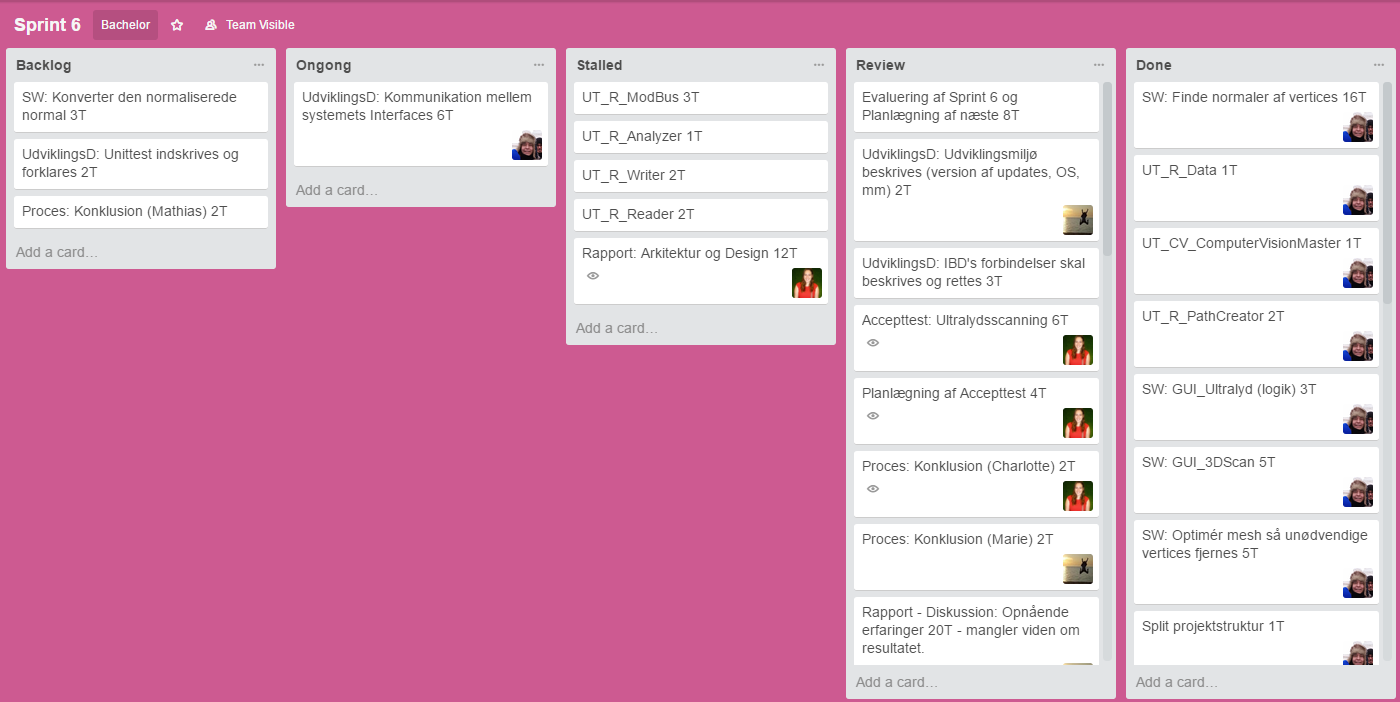
\includegraphics[width=1\textwidth]{figurer/d/Trello}
    \caption{Trello-board fra sprint 6}
    \label{Trello}
\end{figure}

Nedenstående figur \ref{Burn} viser forløbet af sprint 6. Den blå linje er ideelle arbejdetimer, gruppen dagligt skulle nå. Den orange linje er de aktuelle færdiggjorte arbejdstimer. 

\begin{figure}[H]
    \centering
    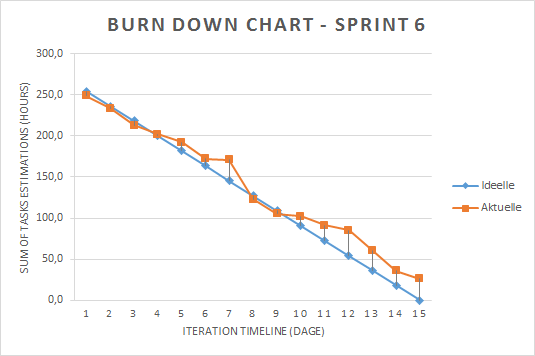
\includegraphics[width=1\textwidth]{figurer/d/Burn-down}
    \caption{Burn-down Chart for sprint 6}
    \label{Burn}
\end{figure}

Som det ses på figur \ref{Burn} ovenfor, når den ideelle linje ikke den aktuelle. Det vil sige, at alle sprintets tasks ikke blev afsluttet. De tasks der ikke blev afsluttet, blev medtaget i sprint 7. 

Efter hvert endt forløb er sprintet evalueret og et nyt er blevet planlagt. I de første 4-5 sprints havde alle gruppens medlemmer undervisning, hvilket har præget, hvordan sprints blev planlagt. Det betød, at nogle tidsbestemmelser ikke var præcise, da det til tider var meget svært at vurdere, hvor meget af gruppens tid der skulle afsættes til øvrige fag - specielt under eksamensperioden. Det gav først mening at tage burn-down charts i brug omkring sprint 5, da gruppen på det tidspunkt var blevet meget bedre til at estimere tasks.

Alle backloggens tasks var indskrevet i Excel, og ved færdiggørelse af en task, blev datoen noteret, og dokumentet opdaterede burn-down chartet. Se bilag \ref{Timebestemt sprints} Timebestemt sprints. 

Det blev besluttet at stoppe brugen af Scrum fra den 9. december, da gruppen vurderede, at det ikke gav mening at tidssætte gennemlæsning af de udviklede dokumenter. Den sidste uge blev brugt på gennemlæsning, ensretning og færdigudvikling af rapport og dokumentation for projektet.  

\textbf{Evaluering af de enkelte sprints} 
Dette afsnit vil kort opsummere de vigtigste punkter for de forskellige sprints. Det har generelt været svært at tidsbestemme ting, som der ikke er erfaring med. Den fulde evaluering af Scrum kan ses i bilag \ref{Evaluering Scrum} Evaluering af Scrum.

Projektforløbet har bestået af syv sprints. Gruppen er for hvert sprint blevet bedre til at strukturere, timebestemme og definere de forskellige tasks. Det første sprint var kort og blev primært brugt til klargøring af projektet og undersøgelse af projekts indhold. Det var først midt i første sprint, at Scrum blev indført. Hidtil havde gruppen anvendt en sekventiel tidsplan, og enkelte opgaver var ikke timebestemte. Ved andet sprint blev det forsøgt at tidsbestemme de forskellige tasks. Generelt for de tidlige sprints endte tasks i kategorien ”stalled”, grundet at tasks var defineret for bredt. Det blev derfor forsøgt at definere tasks med målbare resultater, så det blev muligt at afslutte dem. Undervejs har det været nødvendigt at forlænge enkelte sprints, da gruppens medlemmer havde mere travlt med eksamen end planlagt. Gruppen blev bedre til at tidsbestemme og afslutte tasks, men det var stadig svært at tidsbestemme implementeringsopgaver.

Efter sprint 5 blev det besluttet at opdatere burn-down charts dagligt for at få overblik over sprintenes forløb. Gruppen var blevet bedre til at tidsbestemme hver task, men havde problemer med at opdele tasks i subtasks. På baggrund af den erfaring blev det besluttet, at et task max måtte tage otte timer. Da sprint syv var det sidste sprint, blev nyopståede tasks tilføjet direkte til sprintets backlog, hvilket har betydet at gruppen har arbejdet mere end planlagt.
\newpage
\section{Litteraturstudium}
Litteratursøgning er blevet anvendt ved projektstart til at undersøge bachelorprojektets emne. På dette tidspunt var projektet ikke afgrænset til at omhandle screeningsprogrammet, så der blev søgt bredt for at øge forståelsen for området. Efter møde med Lars Bolvig blev det besluttet, at det ville gavne projektet at undersøge, hvilke konsekvenser en udvidelse af screeningsprogrammet vil medføre. Der er søgt med emneord inden for problemformuleringen i både national og international litteratur på de større databaser (PubMed, Cochrane etc.) for blandt andet at undersøge, om tidlig detektering af brystkræft er rentabel og omkostningseffektiv. Der er yderligere anvendt søgeprotokoller samt Aarhus Universitets online bibliotek til at finde litteratur. Se bilag \ref{Litteraturstudie} Litteraturstudie om screeningsprogrammer for at se hele analysen. 

\section{Møder}
Vejledermøder har været planlagt efter behov, hvor hvert møde typisk har varet en time. Gruppen har sendt en dagsorden til vejleder inden hvert møde, og der er skrevet referat til hvert vejledermøde. Se bilag \ref{Vejledermoder} Vejledermøder.
 
Der har i projektperioden været møder med CEO Søren Pallesen, radiolog og ultralydsekspert Lars Bolvig samt lektor Samuel Alberg Thrysøe. Møder med Søren Pallesen har omhandlet brugen af ultralyd og systemets fremtidige perspektiv. Mødet med Samuel Thrysøe har omhandlet spørgsmål til, hvordan specifikke tests af systemet kunne udføres ved brug af et 3D printet bryst. Møderne med Lars Bolvig har omhandlet teknisk viden omkring utralydsundersøgelser. Se bilag \ref{Eksterne moder} Eksterne møder og bilag \ref{Telefoninterview} Interview med radiolog Lars Bolvig. 

Derudover kontaktede gruppen Tine Bisgaard, som er afdelingsradiograf på Røntgen og skanning, Aarhus Universitetshospital, Tage-Hansens Gade. Tine Bisgaard gav gruppen en rundvisning på afdelingen og efterfølgende et interview. Mødet gav gruppen indsigt i hverdagen på afdelingen, Røntgen og skanning. Se bilag \ref{Tine} Interview med afdelingsradiograf Tine Bisgaard. 

\section{Konflikthåndtering}
Som nævnt tidligere har samarbejdsaftalen været et redskab i forebyggelsen af konflikter. Der har i løbet af projektarbejdet ikke været nogle alvorlige konflikter. De uenigheder, der opstod, blev løst gennem god kommunikation samt forståelse og gensidig respekt for hinandens synspunkter. Uenighederne har typisk omhandlet, hvordan en specifik task eller lignende skulle løses eller beskrives i rapporten. I de tilfælde det har været nødvendigt at inddrage alle gruppens medlemmer for at nå til enighed, bestemte flertallet løsningen. Gruppemedlemmerne er altid nået frem til en løsning, som hele gruppen har været indforstået med. Se bilag \ref{Samarbejdsaftale} Samarbejdsaftale. 

\section{Opnåede erfaringer}
I løbet af projektperioden har gruppen opnået erfaringer inden for agil udvikling, tværfagligt gruppearbejde, kravspecifikation, testspecificering samt produktdokumentation.

Gruppen har opnået erfaring med Scrum som projekstyringsværktøj. Især tidsbestemmelsen og definering af hver task er gruppens medlemmer gradvist blevet bedre til i løbet af hvert sprint. Derudover har gruppen også opnået erfaring prioritering af tasks til sprints, hvilket er gjort ved brug af risikohåndteringen af projektet. Risikohåndteringen har dog ikke kunnet bruges i alle tilfælde, da den blev lavet, før gruppen kendte til alle projektets tasks. Derfor er risikohåndteringen mest blevet anvendt til prioriteringen af tasks i softwareudviklingen, da gruppen her kunne prioritere, hvilke funktionaliteter de fandt vigtigst for Automatisk Ultralydsscanner. 

Gruppen har også opnået erfaringer i formulering og definering af tests til accepttest. Gruppen havde problemer med at få UC3:Hovedscenarie testet. Der blev brugt lang tid på at udtænke en test, som kunne teste Robotarms evne til at følge et bestemt bevægelsesmønster. Gruppen prøvede at teste bevægelsesmønsteret ved at teste med maling, tape og tucsh, samt at beklæde testobjektet med ler for at kunne se Robotarms bevægelsesmønster. 

Derudover har alle gruppens medlemmer opnået vigtig erfaring med tværfagligt samarbejde, hvilket er meget virkelighedsnært i forhold til et kommende arbejde i erhvervslivet. 
Nedenfor har hvert gruppemedlem beskrevet sine opnåede erfaringer med projektarbejdet. 

\textbf{Charlotte Søgaard Kristensen}
Charlotte har i bachelorforløbet fået et større kendskab til projektdokumentation, brugerundersøgelser, økonomi og projektstyring. Charlotte er blevet bedre til LaTeX-redigering i løbet af projektet men har specielt øget sit kendskab til arbejdet med Scrum som projektstyringsværktøj og burn-down chart til at følge processen. Projektstyringen har givet Charlotte en forståelse for planlægning både på lang og kort sigt i et projekt. Det tværfaglige arbejde i forbindelse med bachelorprojektet har givet Charlotte en virkelighedsnær oplevelse af, hvordan det er at arbejde på tværs af professioner. 

\textbf{Marie Kirkegaard}
I bachelorprojektet har Marie lært meget af at lave medicinsk godkendelse af Automatisk Ultralydsscanner. Dette har givet Marie et godt kendskab til Medical Device Directive, samt tilhørende standarder. Derudover har det også givet Marie en forståelse af, hvor omfattende medicinsk godkendelse er for virksomheder. Se bilag \ref{Godkendelsesprocedure} Godkendelsesprocedure, for den medicinske godkendelses. Arbejdet med bachelorprojektet har samtidig givet Marie et godt kendskab til anvendelsen af Scrum som projektstyringsredskab. Marie har også opnået erfaring med tværfagligt arbejde med både Mathias og vejleder, som ikke kommer fra sundhedsteknologi-uddannelsen og derfor er kommet med andre syn på og tilgange til projektarbejde. Arbejdet med bachelorprojektet har også givet Marie et indblik i at udvikle for en kunde med specifikke ønsker til et produkt. 

\textbf{Mathias Siig Nørregaard}
Mathias har fået bedre kendskab til projektarbejdets processer. Selvom Mathias før har prøvet at arbejde med samtlige projekt-elementer (Scrum, kommunikation, tværfaglighed, kravspecifikation, dokumentation osv.), der skulle til for at gennemføre opgaven, er Mathias blevet stærkere på disse områder. Rent teknisk har Mathias opnået erfaring inden for 3D-model teori, som fx udregning af rotationsvektorer, rumtransformation, mesh beregninger m.m. Mathias fik også bedre kendskab til problematikken bag 3D kameraer og robotarme.

\section{Fremtidig arbejdsproces}
I fremtiden kunne det forbedre projektarbejdet, at gruppen blev endnu bedre til at definere de enkelte task i sprintene. Det kunne for eksempel gøres ved at beskrive tasken med et formål samt et omfang. Det samme gælder specifikationen af hvert sprint, hvor gruppen ved sprintets afslutning ville have en bedre forventningsafstemmelse ift. delsystemets udvikling.

Gruppen kunne også have haft fordel af at udføre daglige standup-møder, for at øge forståelsen for andre gruppemedlemmers arbejde.

Det ville også være en fordel for gruppen at bruge en continuous integration testing server. Dette kunne gøres for at gennemføre kontinuerlig og automatisk unit-testing.

Gruppen har også overvejet gruppesammensætningen, da selve udviklingsprocessen ville have gavn af teknisk sparring, hvilket en IKT'er ville kunne have tilført i højere grad end MK og CSK.